\chapter{Study}
Basic stats here:
we ran over X days
over data points

\section{Reader Demographics}

\section{Media Favorability of Candidates}
Each reader was asked to score the five stories according to how favorable each one was to the featured candidate (by headline). 

\begin{figure}[h!] 
\centering
  \fbox{
\includegraphics[width=0.5\textwidth]{favorability_question}}
  \caption{Example of favorability scoring question}
\end{figure}
 
Scores were collected on a three-point scale, Favorable (1), Unfavorable (-1), or Neutral (0).

Overall, media coverage of Trump was viewed as most negatively biased, with over half of stories (51.1\%) viewed as unfavorable towards the candidate.

Of the stories shown, both Sanders and Clinton were viewed as having more positive than negative coverage, at 38.9\% of the 180 annotations being positive. Sanders also had the least negative coverage, with only 18.3\% stories shown being viewed as negatively biased against the candidate. Republican candidate Cruz was also seen to have more negative (33.3\%) than positive (28.9\%) stories about him, although the majority were seen as neutral (37.8\%).

\begin{figure}[h!] 
\centering
  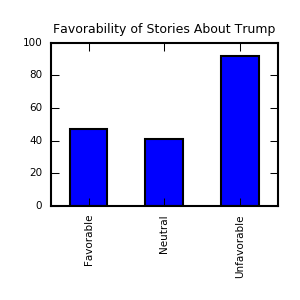
\includegraphics[width=0.24\textwidth]{Trump_favorability} 
  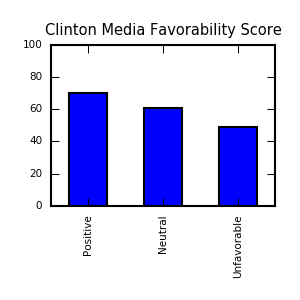
\includegraphics[width=0.24\textwidth]{Clinton_favorability} 
  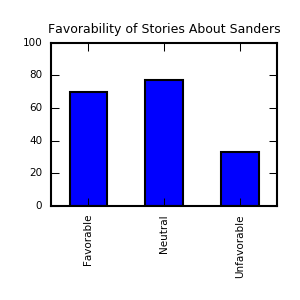
\includegraphics[width=0.24\textwidth]{Sanders_favorability} 
  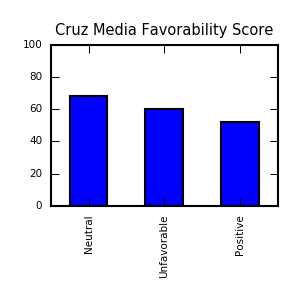
\includegraphics[width=0.24\textwidth]{Cruz_favorability} 
  \caption{Media Favorability of Candidates}
\end{figure}
 


WHAT ABOUT IN COMPARISON TO TRUSTWORTHINESS THO?
WHEN WE LOOK AT ONLY TRUSTWORTHY STORIES

 

Bernie Sanders
 0    42.777778
 1    38.888889
-1    18.333333
Name: favor, dtype: float64

Hillary Clinton
 1    38.888889
 0    33.888889
-1    27.222222
Name: favor, dtype: float64

Ted Cruz
 0    37.777778
-1    33.333333
 1    28.888889
Name: favor, dtype: float64


\section{Overall Bias Reportings}


% This is an example of how you would use tgrind to include an example
% of source code; it is commented out in this template since the code
% example file does not exist.  To use it, you need to remove the '%' on the
% beginning of the line, and insert your own information in the call.
%
%\tagrind[htbp]{code/pmn.s.tex}{Post Multiply Normalization}{opt:pmn}
 